\section{Are there grandmother cells in CNNs?}
\label{sec:grand-mother}
Neuroscientists have conjectured that cells in the human brain which only respond to very specific and complex visual stimuli (such as the face of one's grandmother) are involved in object recognition.
These neurons are often referred to as \emph{grandmother cells} (GMC) \cite{Barlow,Grandmother}. 
Proponents of artificial neural networks have shown great interest in reporting the presence of GMC-like filters for specific object classes in their networks (see, for example, the cat filter reported in \cite{GoogleCat}). 
The notion of GMC like features is also related to standard feature encodings for image classification.
Prior to the work of \cite{Kriz}, the dominant approaches for image and scene classification were based on either representing images as a bag of local descriptors (BoW), such as SIFT (e.g., \cite{lazebnik2006beyond}), or by first finding a set of mid-level patches \cite{Blocks,Mid1} and then encoding images in terms of them. 
The problem of finding good mid-level patches is often posed as a search for a set of high-recall discriminative templates. 
In this sense, mid-level patch discovery is the search for a set of GMC templates. 
The low-level BoW representation, in contrast, is a \emph{distributed code} in the sense that a single feature by itself is not discriminative, but a group of features taken together is.
This makes it interesting to investigate the nature of mid-level CNN features such as conv-5. 

%Recently, proponents of artificial neural networks have shown great interest in reporting the presence of GMC-like filters for specific object classes in their networks (see, for example, the cat filter reported in \cite{GoogleCat}). 
For understanding these feature representations in CNNs, \cite{Simonyan,DeConv} recently presented methods for finding locally optimal visual inputs for individual filters.
%These methods isolate individual inputs that activate a filter, but do not characterize the \emph{distribution} of images that cause an individual filter to fire above a certain threshold. \todo{make this argument clearer}.
However, these methods only find the best, or in some cases top-$k$, visual inputs that activate a filter, but do not characterize the \emph{distribution} of images that cause an individual filter to fire above a certain threshold. For example, if it is found that the top-10 visual inputs for a particular filter are cats, it remains unclear what is the response of the filter to other images of cats.
Thus, it is not possible to make claims about presence of GMC like filters for cat based on such analysis. 
A GMC filter for the cat class, is one that fires strongly on \emph{all} cats and nothing else.
%If, for example, we wish to see if the network contains a GMC filter for the \emph{cat} class, then we should look for a particular filter that fires strongly on all cats and nothing else.
This criteria can be expressed as a filter that has high \emph{precision} and high \emph{recall}.
That is, a GMC filter for class $C$ is a filter that has a high average precision (AP) when tasked with classifying inputs from class $C$ versus inputs from all other classes.

%Mathematically, this computation is expressed as finding the set of images $\mathcal{I}$ which maximally activate a single feature (i.e. find $i \in \mathcal{I}$ s.t. Feature-score(i) $\geq th$ $\forall i $, where $th$ is a threshold value). The distribution of class labels associated with this set of images ($\mathcal{I}$), defines the \textit{precision} of the feature. However, this distribution does not account for the \textit{recall}.  The presence/absence of GMC is a scientifically interesting question to pursue, but for recognition, we require features with both high precision and high recall. Consequently, we argue that if the goal is object recognition, then GMC for a particular object class should be interpreted as features with high AP and not just high precision. 
 
%Further, the notion of GMC-like features is related to standard feature encodings for image classification.
%Prior to the work of \cite{Kriz}, the dominant approaches for image and scene classification were based on either representing images as a bag of local descriptors (BoW), such as SIFT (e.g., \cite{lazebnik2006beyond}), or by first finding a set of mid-level patches \cite{Blocks,Mid1} and then encoding images in terms of them. 
%The problem of finding good mid-level patches is often posed as a search for a set of high-recall discriminative templates. 
%In this sense, mid-level patch discovery is the search for a set of GMC templates. 
%The low-level BoW representation, in contrast, is a \emph{distributed code} in the sense that a single feature by itself is not discriminative, but a group of features taken together is.
%This makes it interesting to investigate the nature of mid-level CNN features such as conv-5. 

First, we address the question of finding GMC filters by computing the AP of individual filters (Section \ref{sub:class-specific-unit}). Next, we measure how distributed are the feature representations (Section \ref{sub:how-many}). For both experiments we use features from layer conv-5, which consists of responses of 256 filters in a $6\times 6$ spatial grid. Using max pooling, we collapse the spatial grid into a 256-D vector, so that for each filter we have a single response per image (in Section \ref{sub:imp-mag} we show that this transformation causes only a small drop in task performance).

%The output of conv-5 is the response of 256 filters in a $6\times 6$ spatial grid which we collapse into a 256-D vector using max-pooling (see section \ref{sub:imp-loc} for more details)

\setlength{\unitlength}{\linewidth}
\begin{figure}[t!]
\centering
%\subfloat{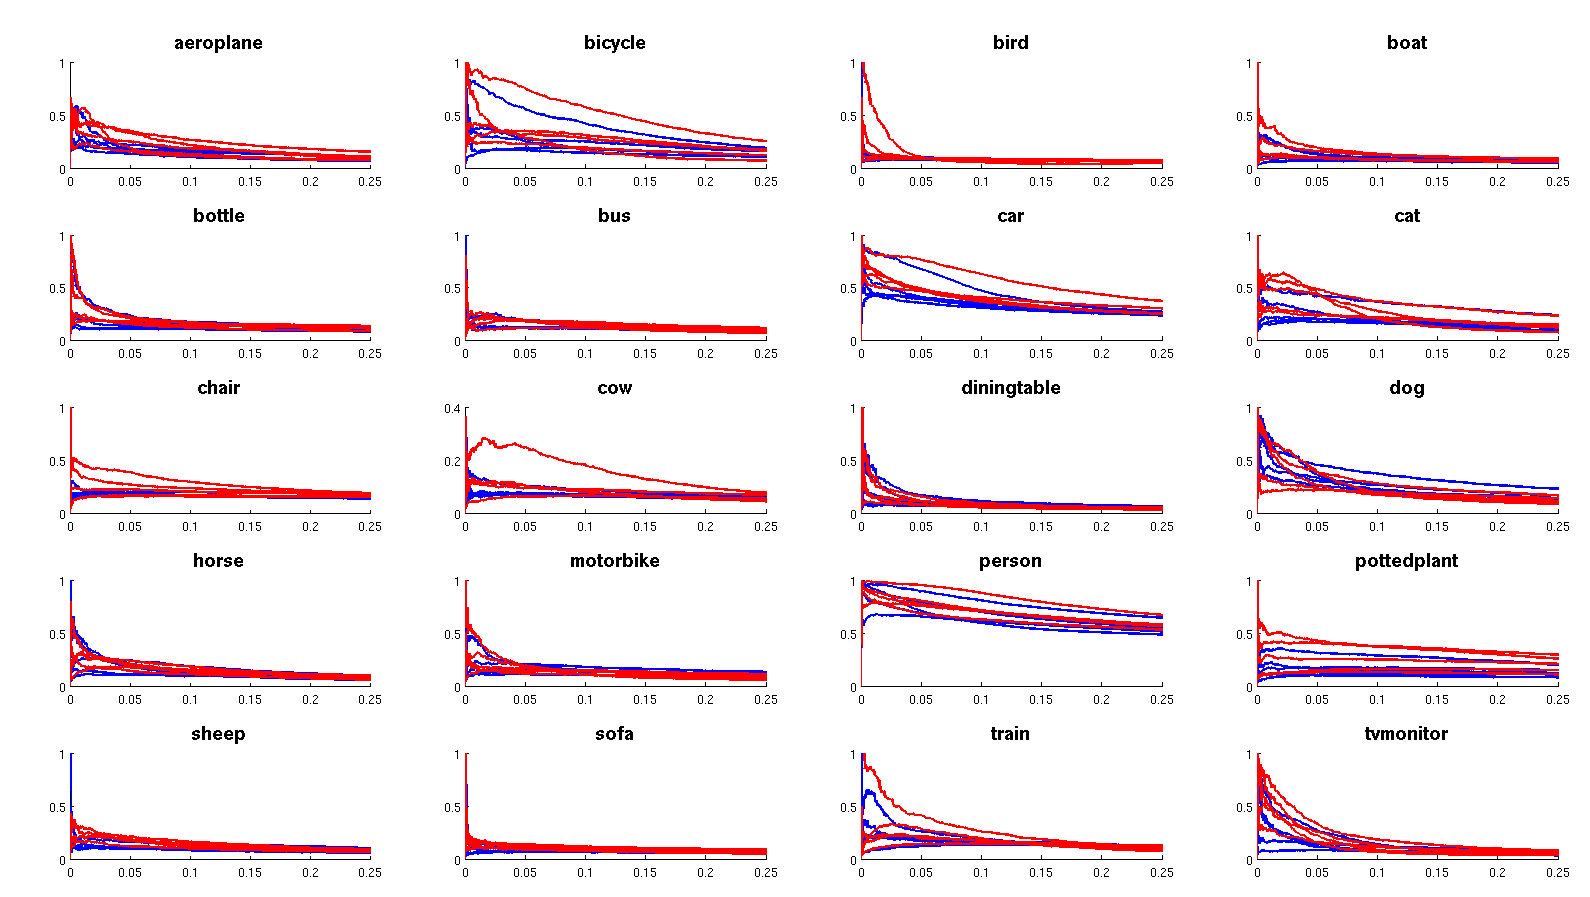
\includegraphics[scale=0.20]{images/gtbbox_pascal_prerec_pool5units.png}}
\begin{picture}(0.04,0.3)(0,0)
\put(0.0,0.20){\rotatebox{90}{\scriptsize{\textbf{Precision}}}}
\end{picture}
\subfloat{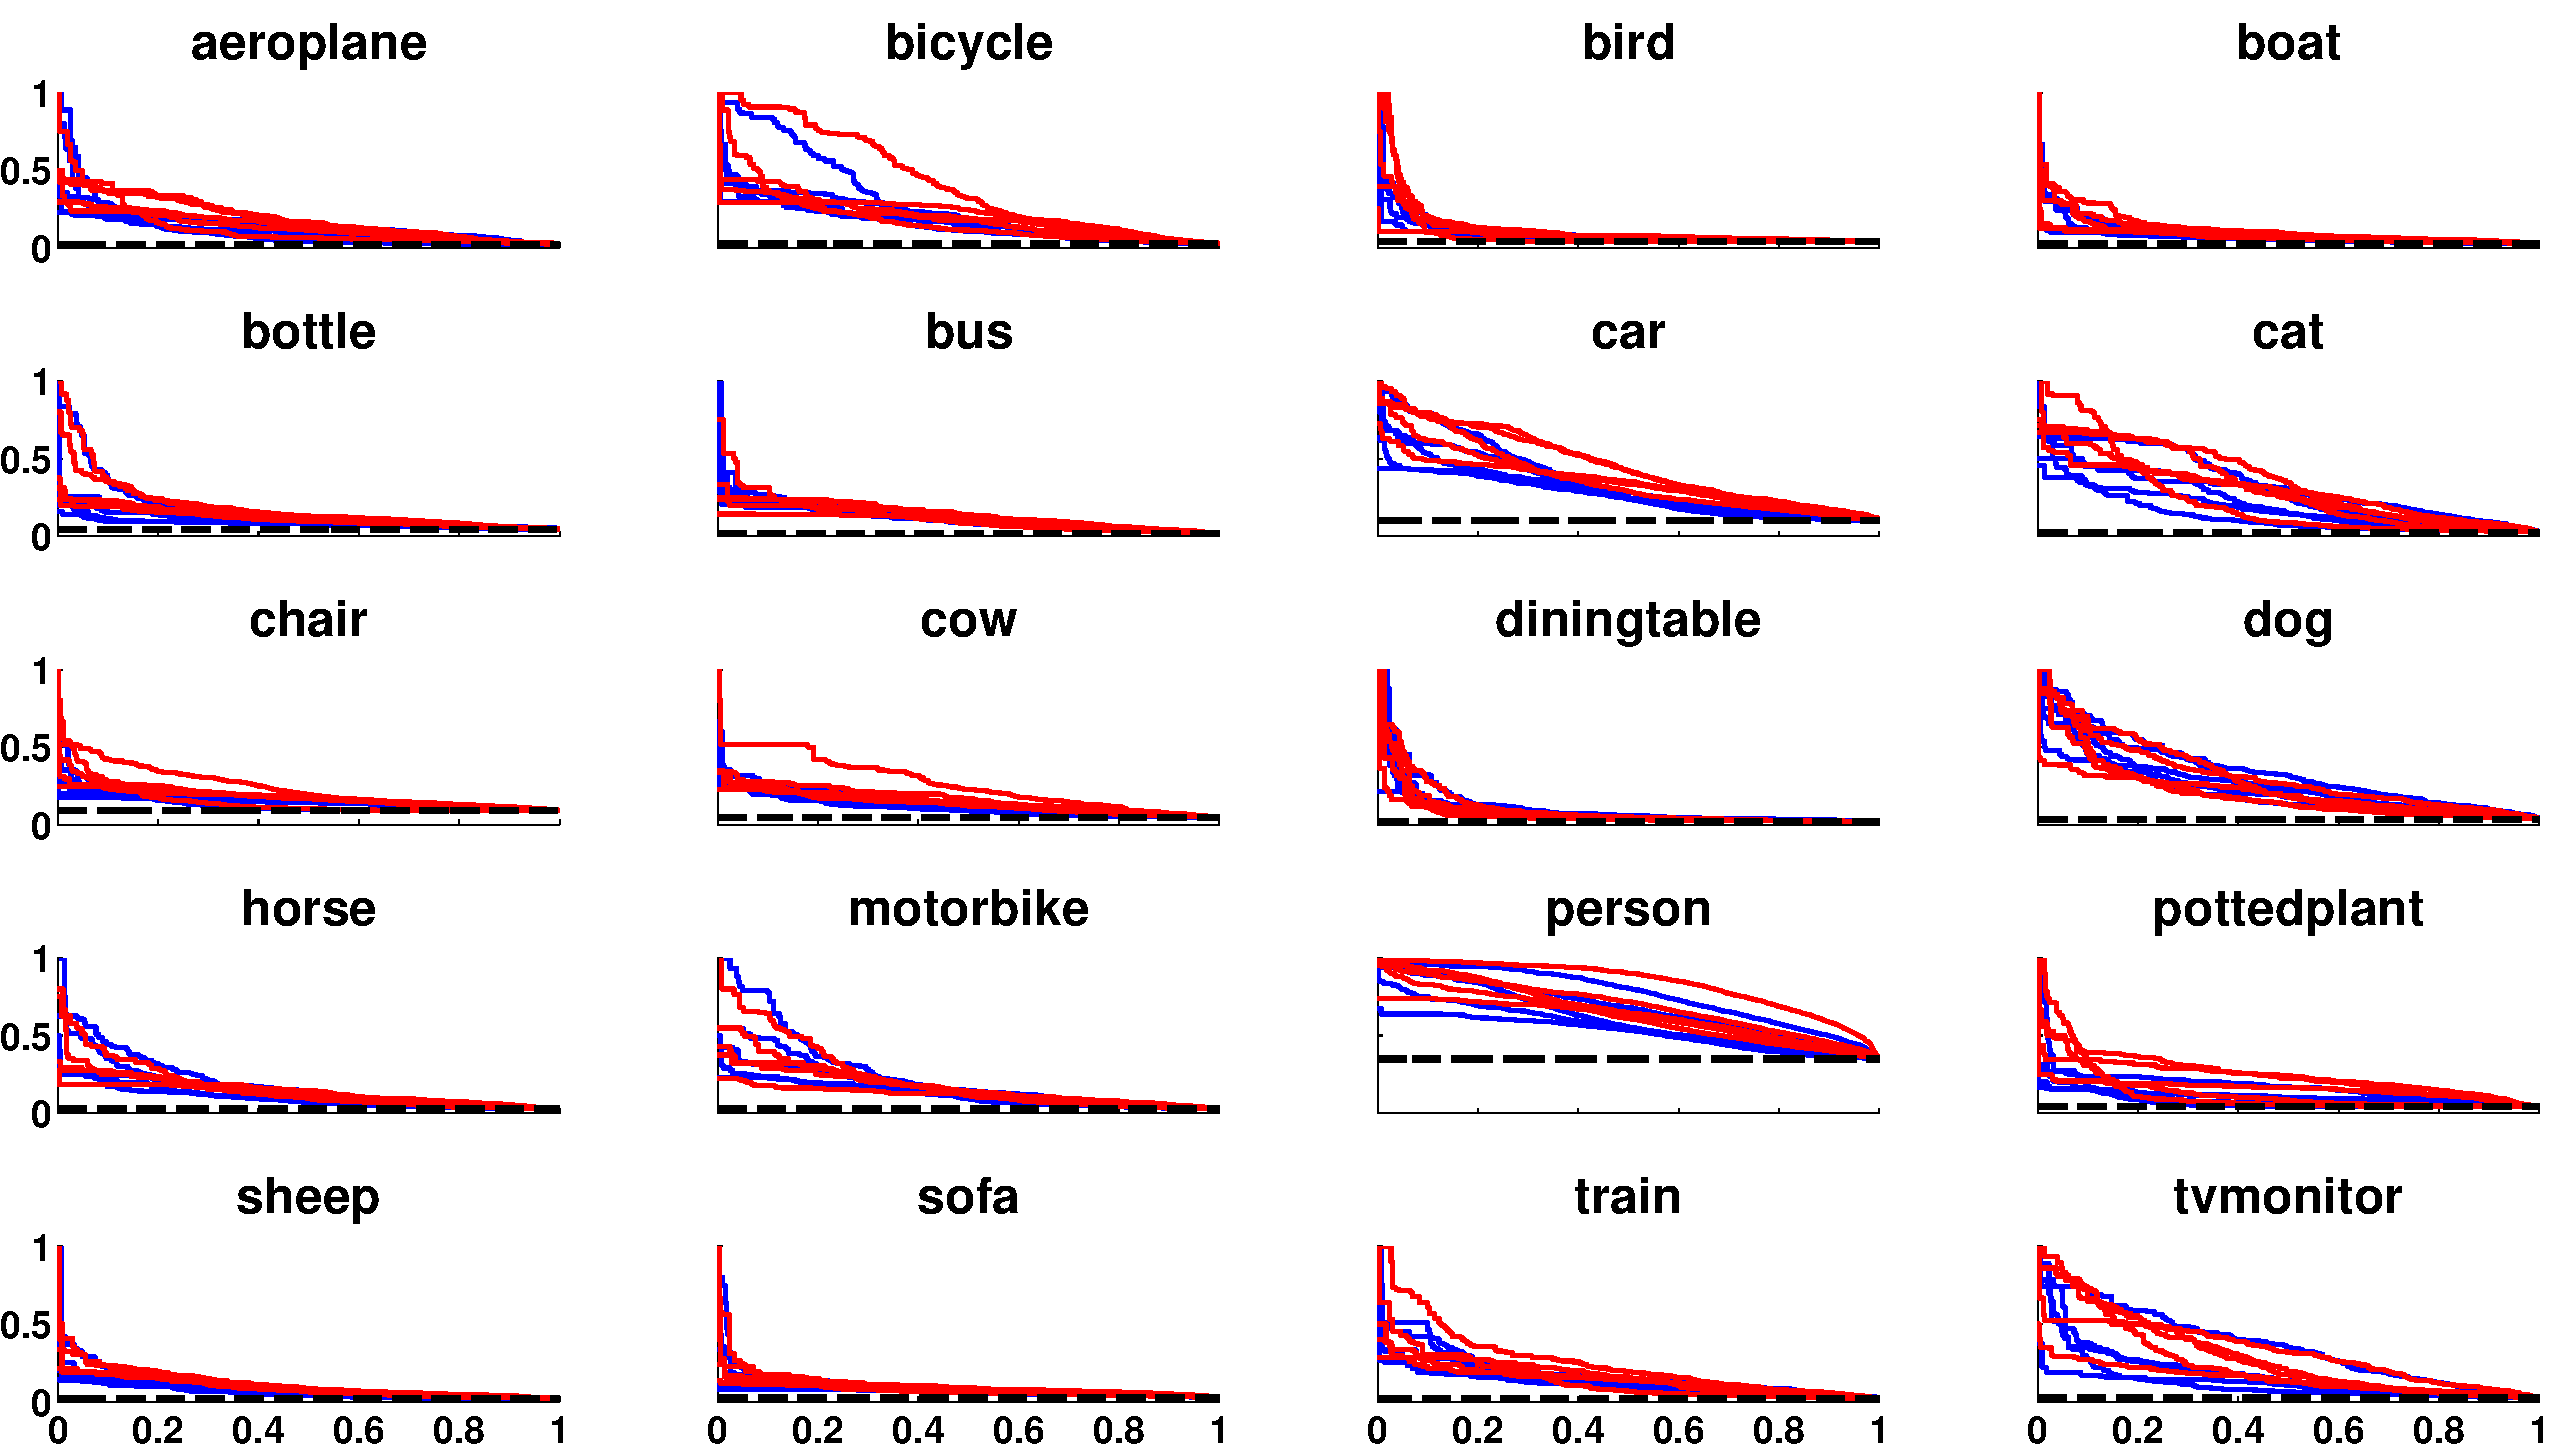
\includegraphics[width=0.93\linewidth]{images/pool5_ap_filters.pdf}} \vspace{0.4mm}
\begin{picture}(1.0,0.01)(0,0)
\put(0.50,0.0){{\scriptsize{\textbf{Recall}}}}
\end{picture}
\caption{The precision-recall curves for the top five (based on AP) conv-5 filter responses on PASCAL-DET-GT. Curves in red and blue indicate AP for fine-tuned and pre-trained networks, respectively. The dashed black line is the performance of a random filter. For most classes, precision drops significantly even at modest recall values. There are GMC filters for classes such as bicycle, person, car, cat.}
\label{fig:ap}
\end{figure}

\subsection{Finding Grandmother Cells}
\label{sub:class-specific-unit}
For each filter, its AP value is calculated for classifying images using class labels and filter responses to object bounding boxes from PASCAL-DET-GT. Then, for each class we sorted filters in decreasing order of their APs. If GMC filters for this class exist, they should be the top ranked filters in this sorted list. The precision-recall curves for the top-five conv-5 filters are shown in Figure \ref{fig:ap}. We find that GMC-like filters exist for only for a few classes, such as bicycle, person, cars, and cats.


%\begin{figure}[t!]
%\centering
%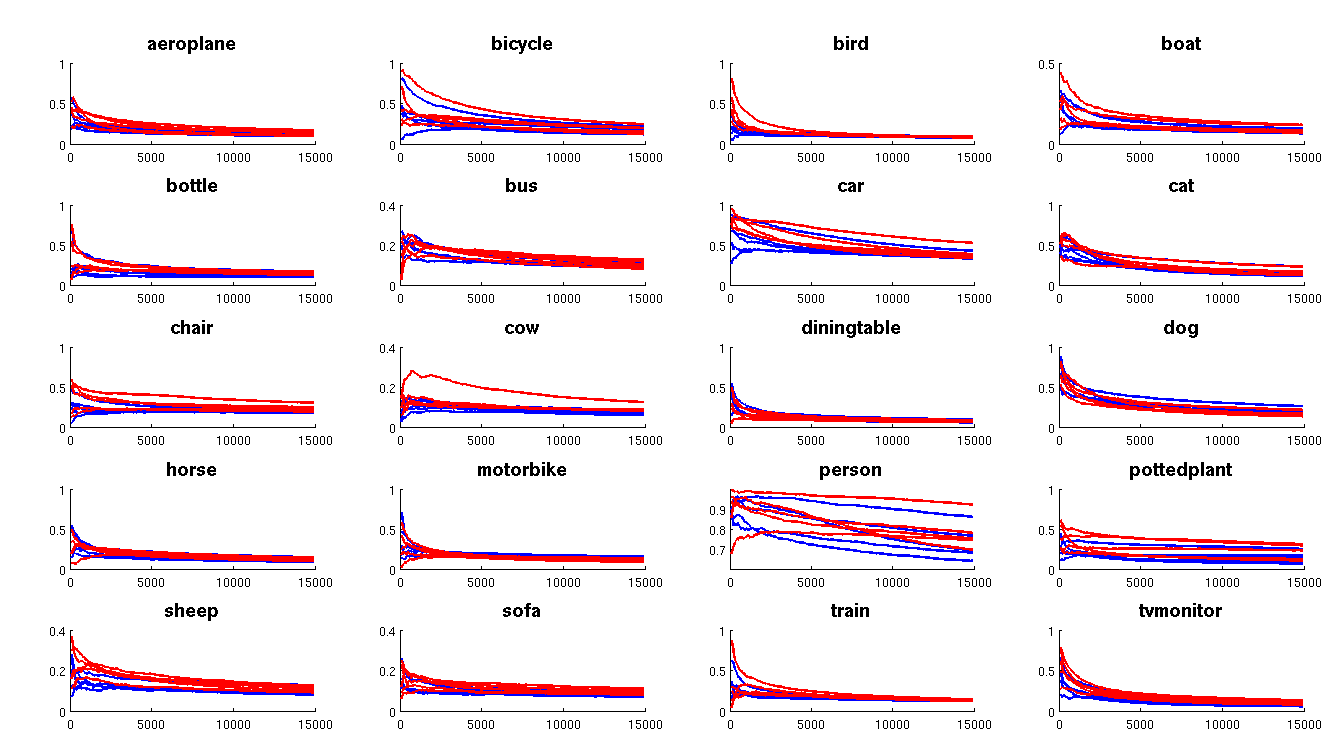
\includegraphics[scale=0.20]{images/prob_sel_dims_top5.png}
%\caption{This plot shows the precision curve for the top 5 most selective filters taken from Alex-Net (Blue) and FT-Net(Red) for all PASCAL classes. Y-axis is the precision and X-axis is number of examples.}
%\label{fig:prob-sel}
%\end{figure}

\subsection{How distributed are the feature representations?}
\label{sub:how-many}

%\begin{comment}
%\begin{figure}[t!]
%\centering
%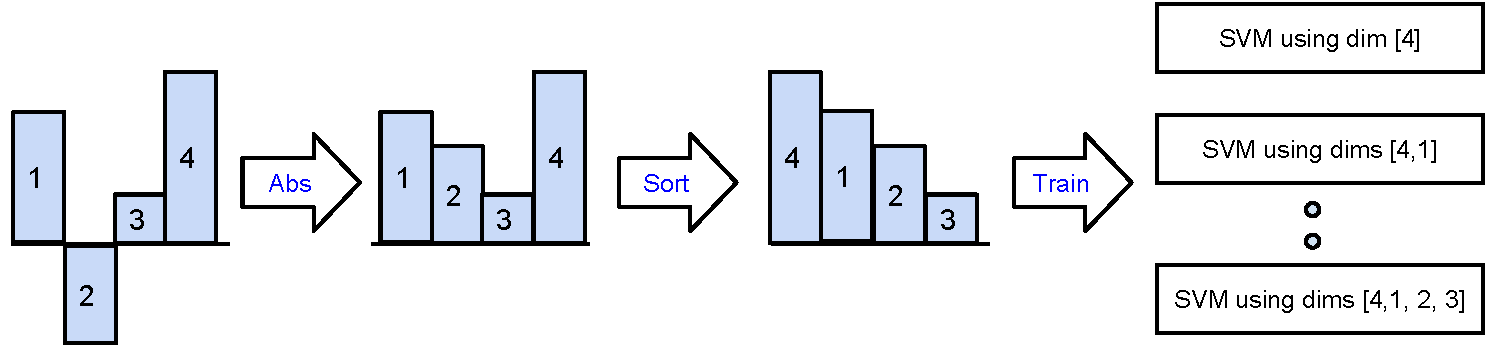
\includegraphics[scale=0.35]{images/how-many.pdf}
%\caption{Illustrating the greedy strategy used for selecting filters. First, linear SVM is trained to classify images of particular classes from 256-D conv-5 responses. The magnitudes of individual dimensions of the learnt SVM weight vectors are used as a proxy for determining the importance of each dimension. For the sake of clarity, this procedure is described using a 4-D weight vector shown on the extreme left (the numbers on each bar are the dimension). Firstly, we take the absolute value for each dimension and then sort the dimensions based on this value. Then, we chose the top k filters/dimensions from this ranked list to construct a subset of size k.}
%%\caption{Illustration of the greedy strategy used for selecting filters. For each class, a linear SVM is trained after ``sp-max'' feature transformation described in section \ref{sub:imp-loc} is applied. ``sp-max''  reduces conv-5 features into a 256-D vector, wherein each dimension corresponds to one of the 256 conv-5 filters. The magnitude of individual dimensions of the weight vector learned by SVM is used as a proxy for determining the importance of each dimension. For the sake of clarity, this procedure is described using a 4-D weight vector shown on the extreme left (the numbers on each bar are the dimension). Firstly, we take the absolute value for each dimension and then sort the dimensions based on this value. Then, we chose the top k filters/dimensions from this ranked list to construct a subset of size k.}
%\label{fig:sel-strategy}
%\end{figure}
%\end{comment}

In addition to visualizing the AP curves of individual filters, we measured the number of filters required to recognize objects of a particular class. 
%Feature selection was performed to construct nested subsets of filters, ranging from a single filter to all filters, using the greedy strategy described in Figure \ref{fig:sel-strategy}.\footnote{Filter subsets of size [1, 2, 3, 5, 10, 15, 20, 25, 30, 35, 40, 45, 50, 80, 100, 128, 256] were used.}
Feature selection was performed to construct nested subsets of filters, ranging from a single filter to all filters, using the following greedy strategy. First, separate linear SVMs were trained to classify object bounding boxes from PASCAL-DET-GT using conv-5 responses. 
For a given class, the 256 dimensions of the learnt weight vector ($w$) is in direct correspondence with the 256 conv-5 filters. We used the magnitude of the $i$-th dimension of $w$ to rank the importance of the $i$-th conv-5 filter for discriminating instances of this class. 
Next, all filters were sorted using these magnitude values. Each subset of filters was constructed by taking the top-$k$ filters from this list.\footnote{We used values of $k \in \{1, 2, 3, 5, 10, 15, 20, 25, 30, 35, 40, 45, 50, 80, 100, 128, 256\}$.} For each subset, a linear SVM was trained using only the responses of filters in that subset for classifying the class under consideration.

\setlength{\unitlength}{\linewidth}
\begin{figure}[t!]
\centering
%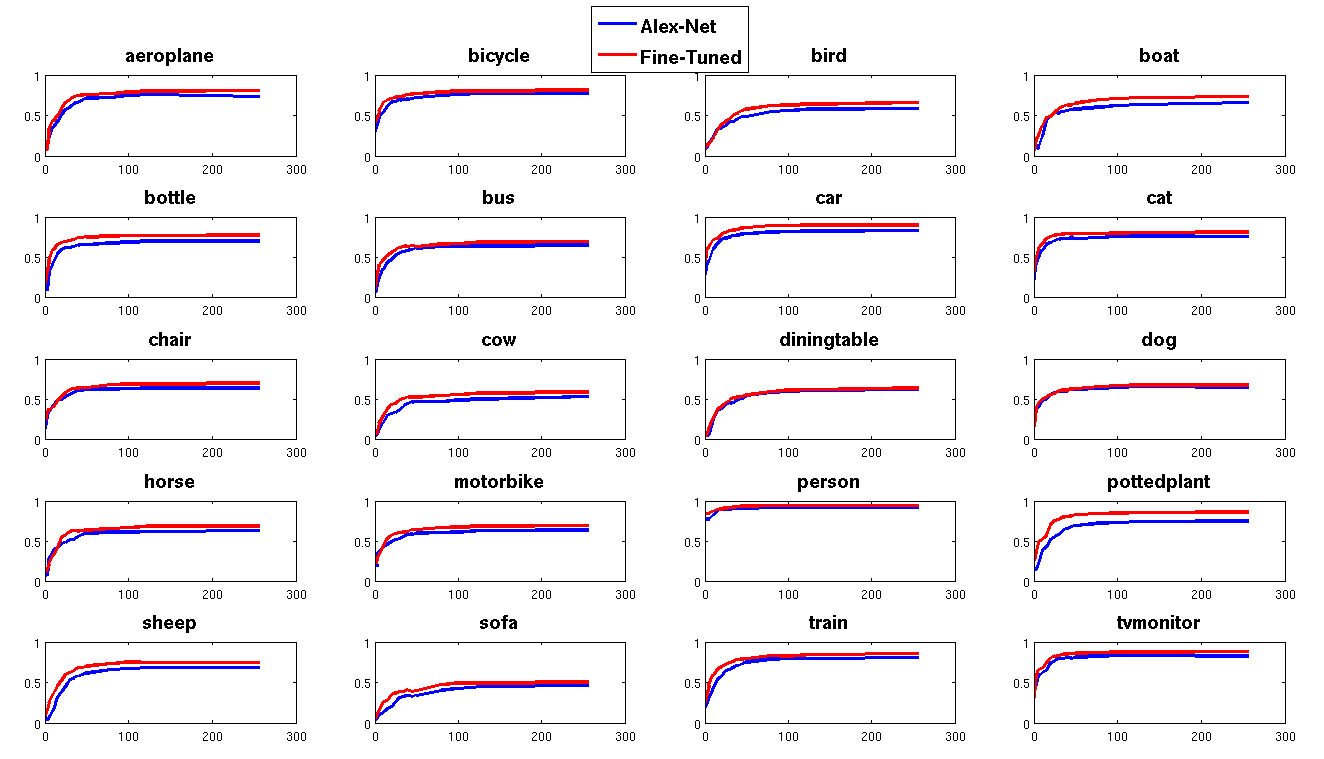
\includegraphics[height=6.5cm]{images/svm_seldims.png}
\begin{picture}(0.04,0.3)(0,0)
\put(0.0,0.06){\rotatebox{90}{\scriptsize{\textbf{Fraction of complete performance}}}}
\end{picture}
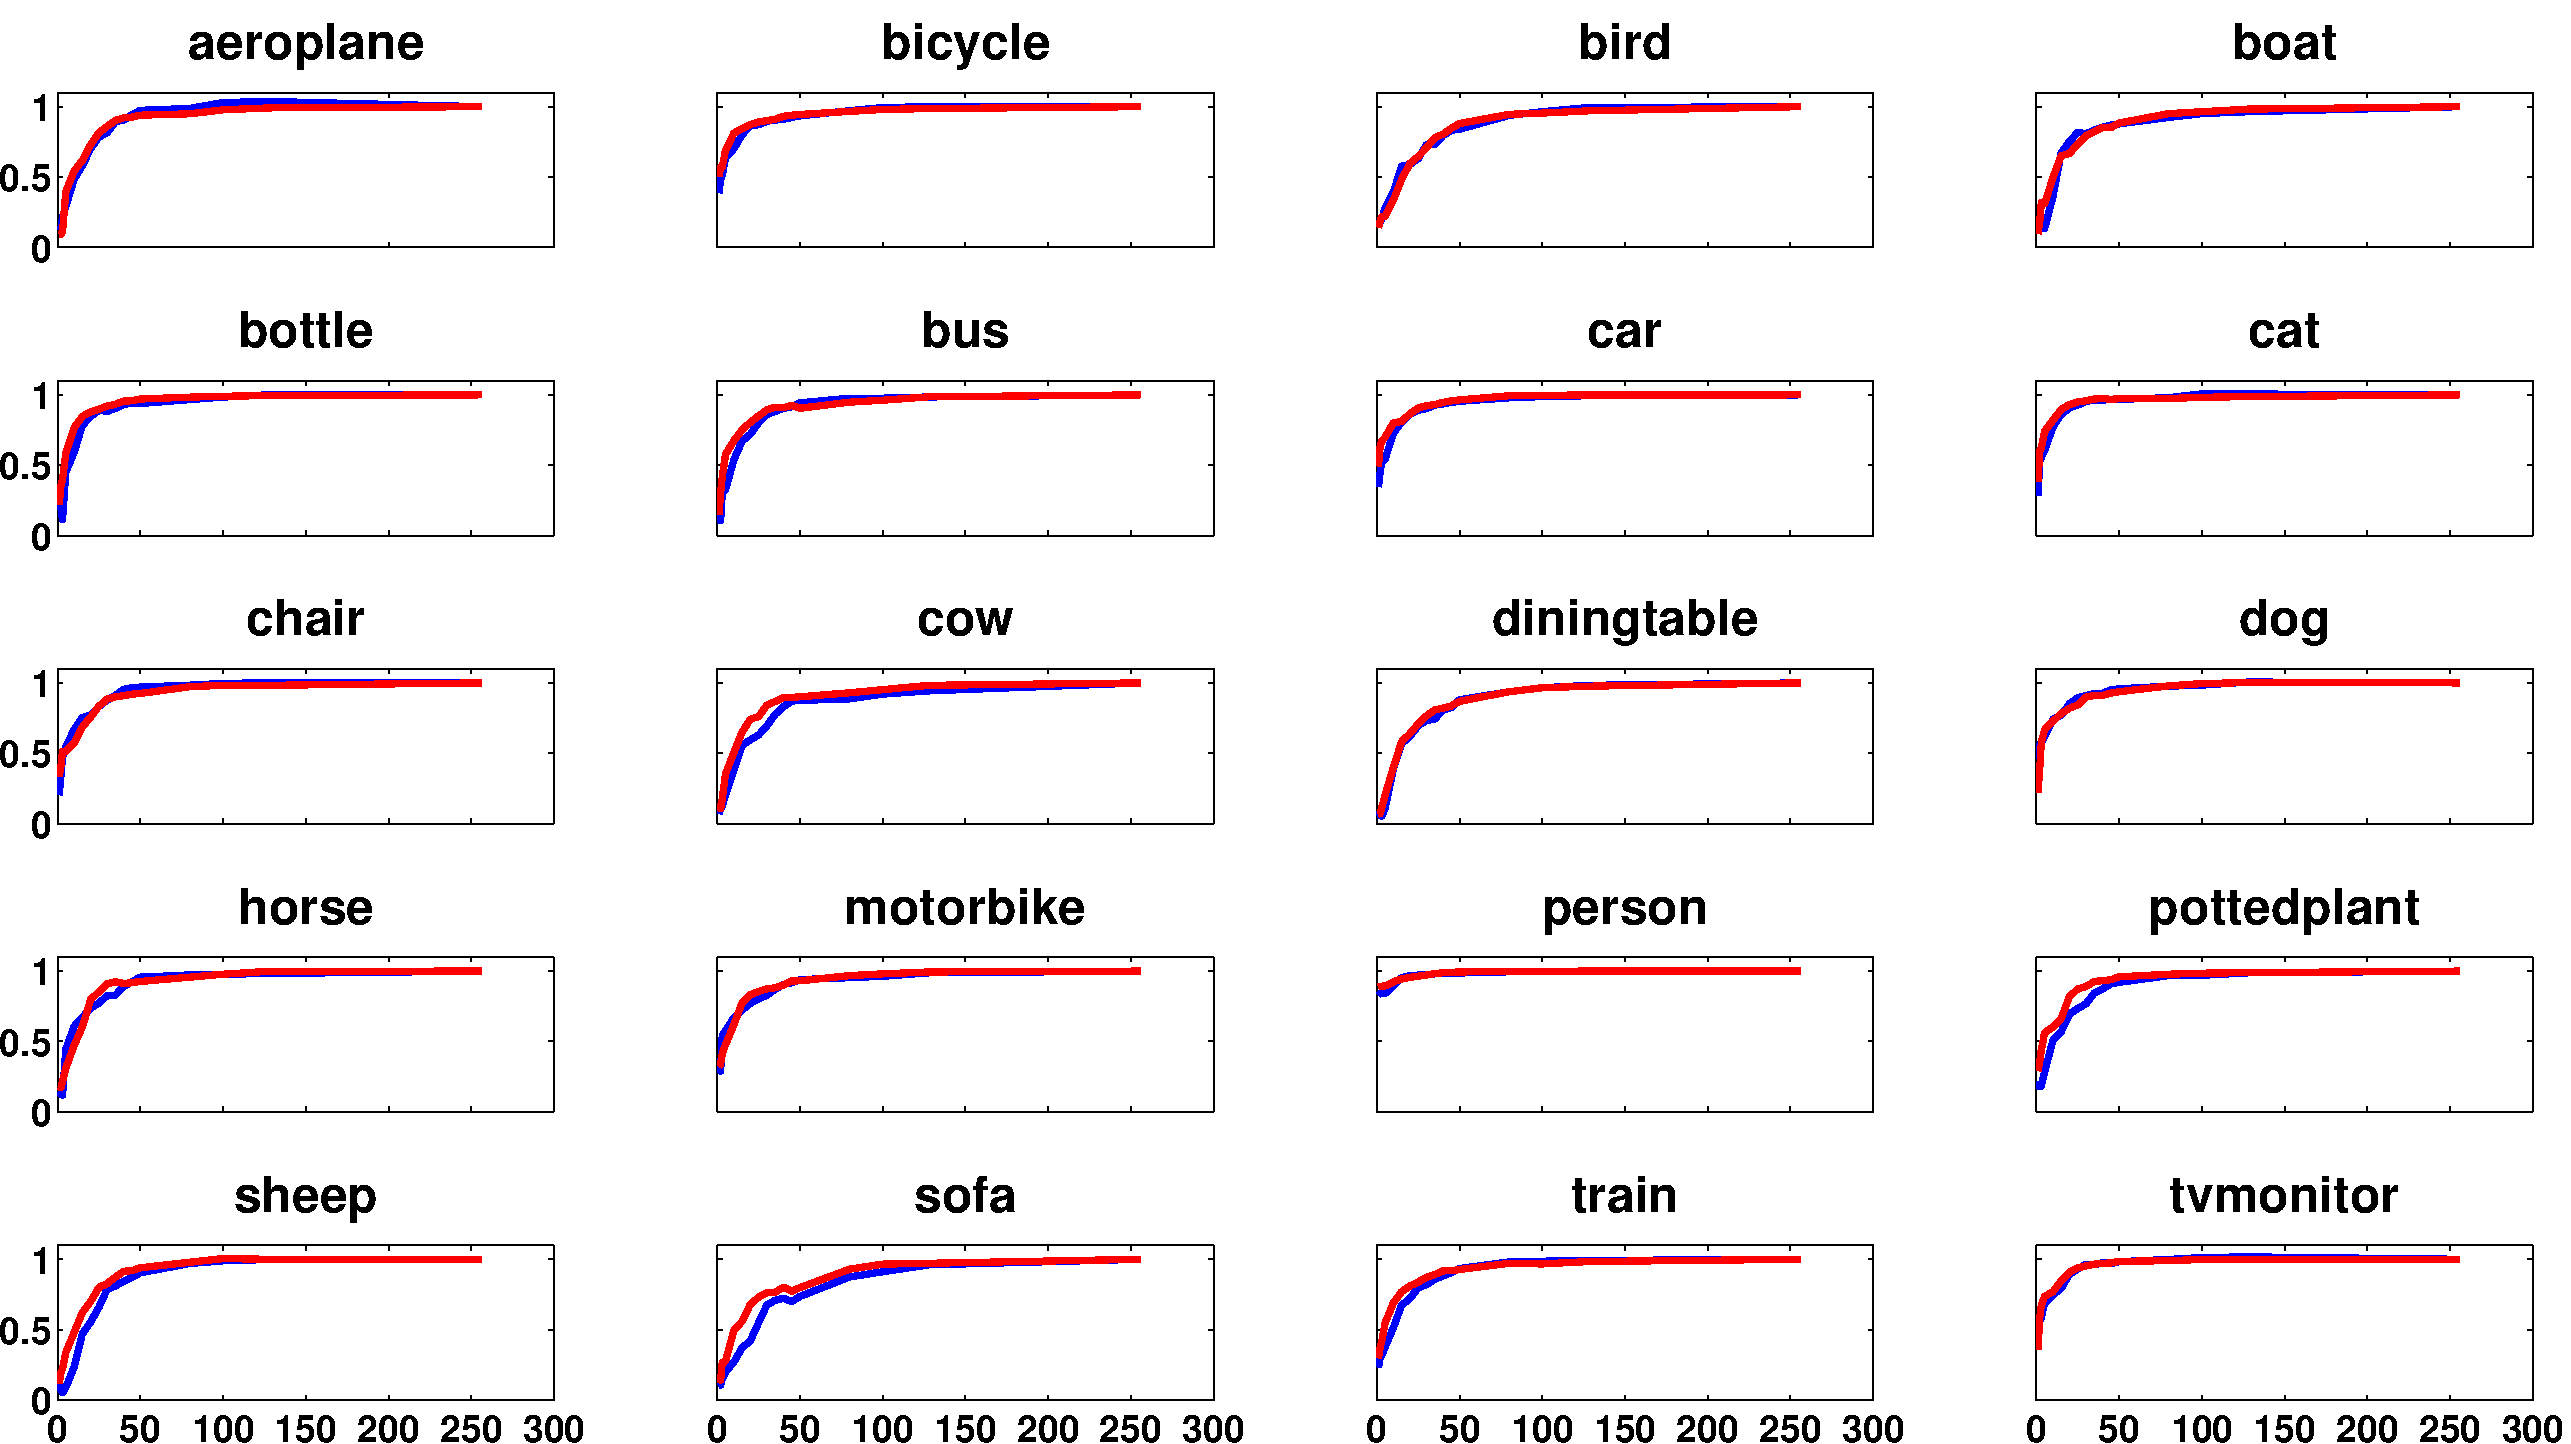
\includegraphics[width=0.93\linewidth]{images/pool5_spmax_num_svm_filters.pdf}
\begin{picture}(1.0,0.01)(0,0)
\put(0.40,0.0){{\scriptsize{\textbf{Number of conv-5 filters}}}}
\end{picture}
\caption{The fraction of complete performance on PASCAL-DET-GT achieved by conv-5 filter subsets of different sizes. Complete performance is the AP computed by considering responses of all the filters. Notice, that for a few classes such as person and bicycle only a few filters are required, but for most classes substantially more filters are needed, indicating a distributed code.}
\label{fig:svm-sel-dims}
\end{figure}  

\setlength{\tabcolsep}{1.1pt}
\begin{table}[t!]
\renewcommand{\arraystretch}{1.2}
\begin{center}
\caption{Number of filters required to achieve 50\% or 90\% of the complete performance on PASCAL-DET-GT using a CNN pre-trained on ImageNet and fine-tuned for PASCAL-DET using conv-5 features.}
\label{table:num-fil}
\resizebox{\linewidth}{!}{
\begin{tabular}{l|c||cccccccccccccccccccc}
\noalign{\smallskip}
& perf. & aero & bike & bird & boat & bottle & bus & car & cat & chair & cow & table & dog & horse & mbike & person & plant & sheep & sofa & train & tv \\
\hline
pre-train & 50\% & 15 & 3 & 15 & 15 & 10 & 10 & 3 & 2 & 5 & 15 & 15 & 2 & 10 & 3 & 1 & 10 & 20 & 25 & 10 & 2 \\ 
fine-tune & 50\% & 10 & 1 & 20 & 15 & 5 & 5 & 2 & 2 & 3 & 10 & 15 & 3 & 15 & 10 & 1 & 5 & 15 & 15 & 5 & 2 \\
\hline
pre-train & 90\% & 40 & 35 & 80 & 80 & 35 & 40 & 30 & 20 & 35 & 100 & 80 & 30 & 45 & 40 & 15 & 45 & 50 & 100 & 45 & 25 \\
fine-tune & 90\% & 35 & 30 & 80 & 80 & 30 & 35 & 25 & 20 & 35 & 50 & 80 & 35 & 30 & 40 & 10 & 35 & 40 & 80 & 40 & 20 \\
\end{tabular}
}
\end{center}
\end{table}
\setlength{\tabcolsep}{1.4pt}
  
The variation in performance with the number of filters is shown in Figure \ref{fig:svm-sel-dims}.
Table \ref{table:num-fil} lists the number of filters required to achieve 50\% and 90\% of the complete performance. For classes such as persons, cars, and cats relatively few filters are required, but for most classes around 30 to 40 filters are required to achieve at least 90\% of the full performance. This indicates that the conv-5 feature representation is distributed and there are GMC-like filters for only a few classes.
Results using layer fc-7 are presented in the the supplementary material.
We also find that after fine-tuning, slightly fewer filters are required to achieve performance levels similar to a pre-trained network. 

\begin{figure}[t!]
\centering
%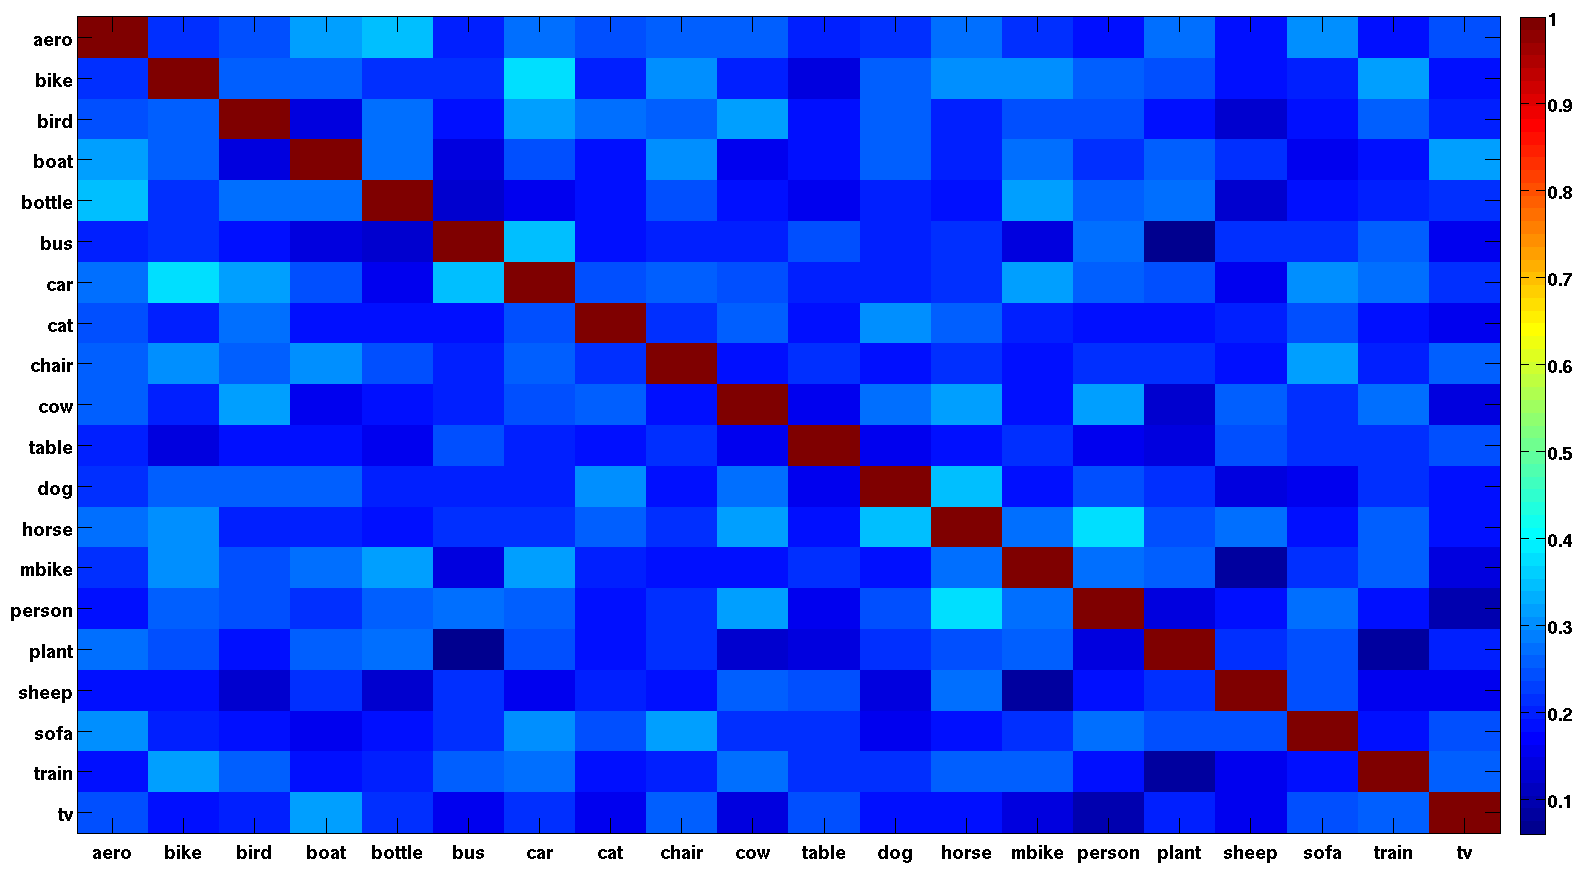
\includegraphics[width=1.0\linewidth]{images/ftNet_commonfilters.png}
%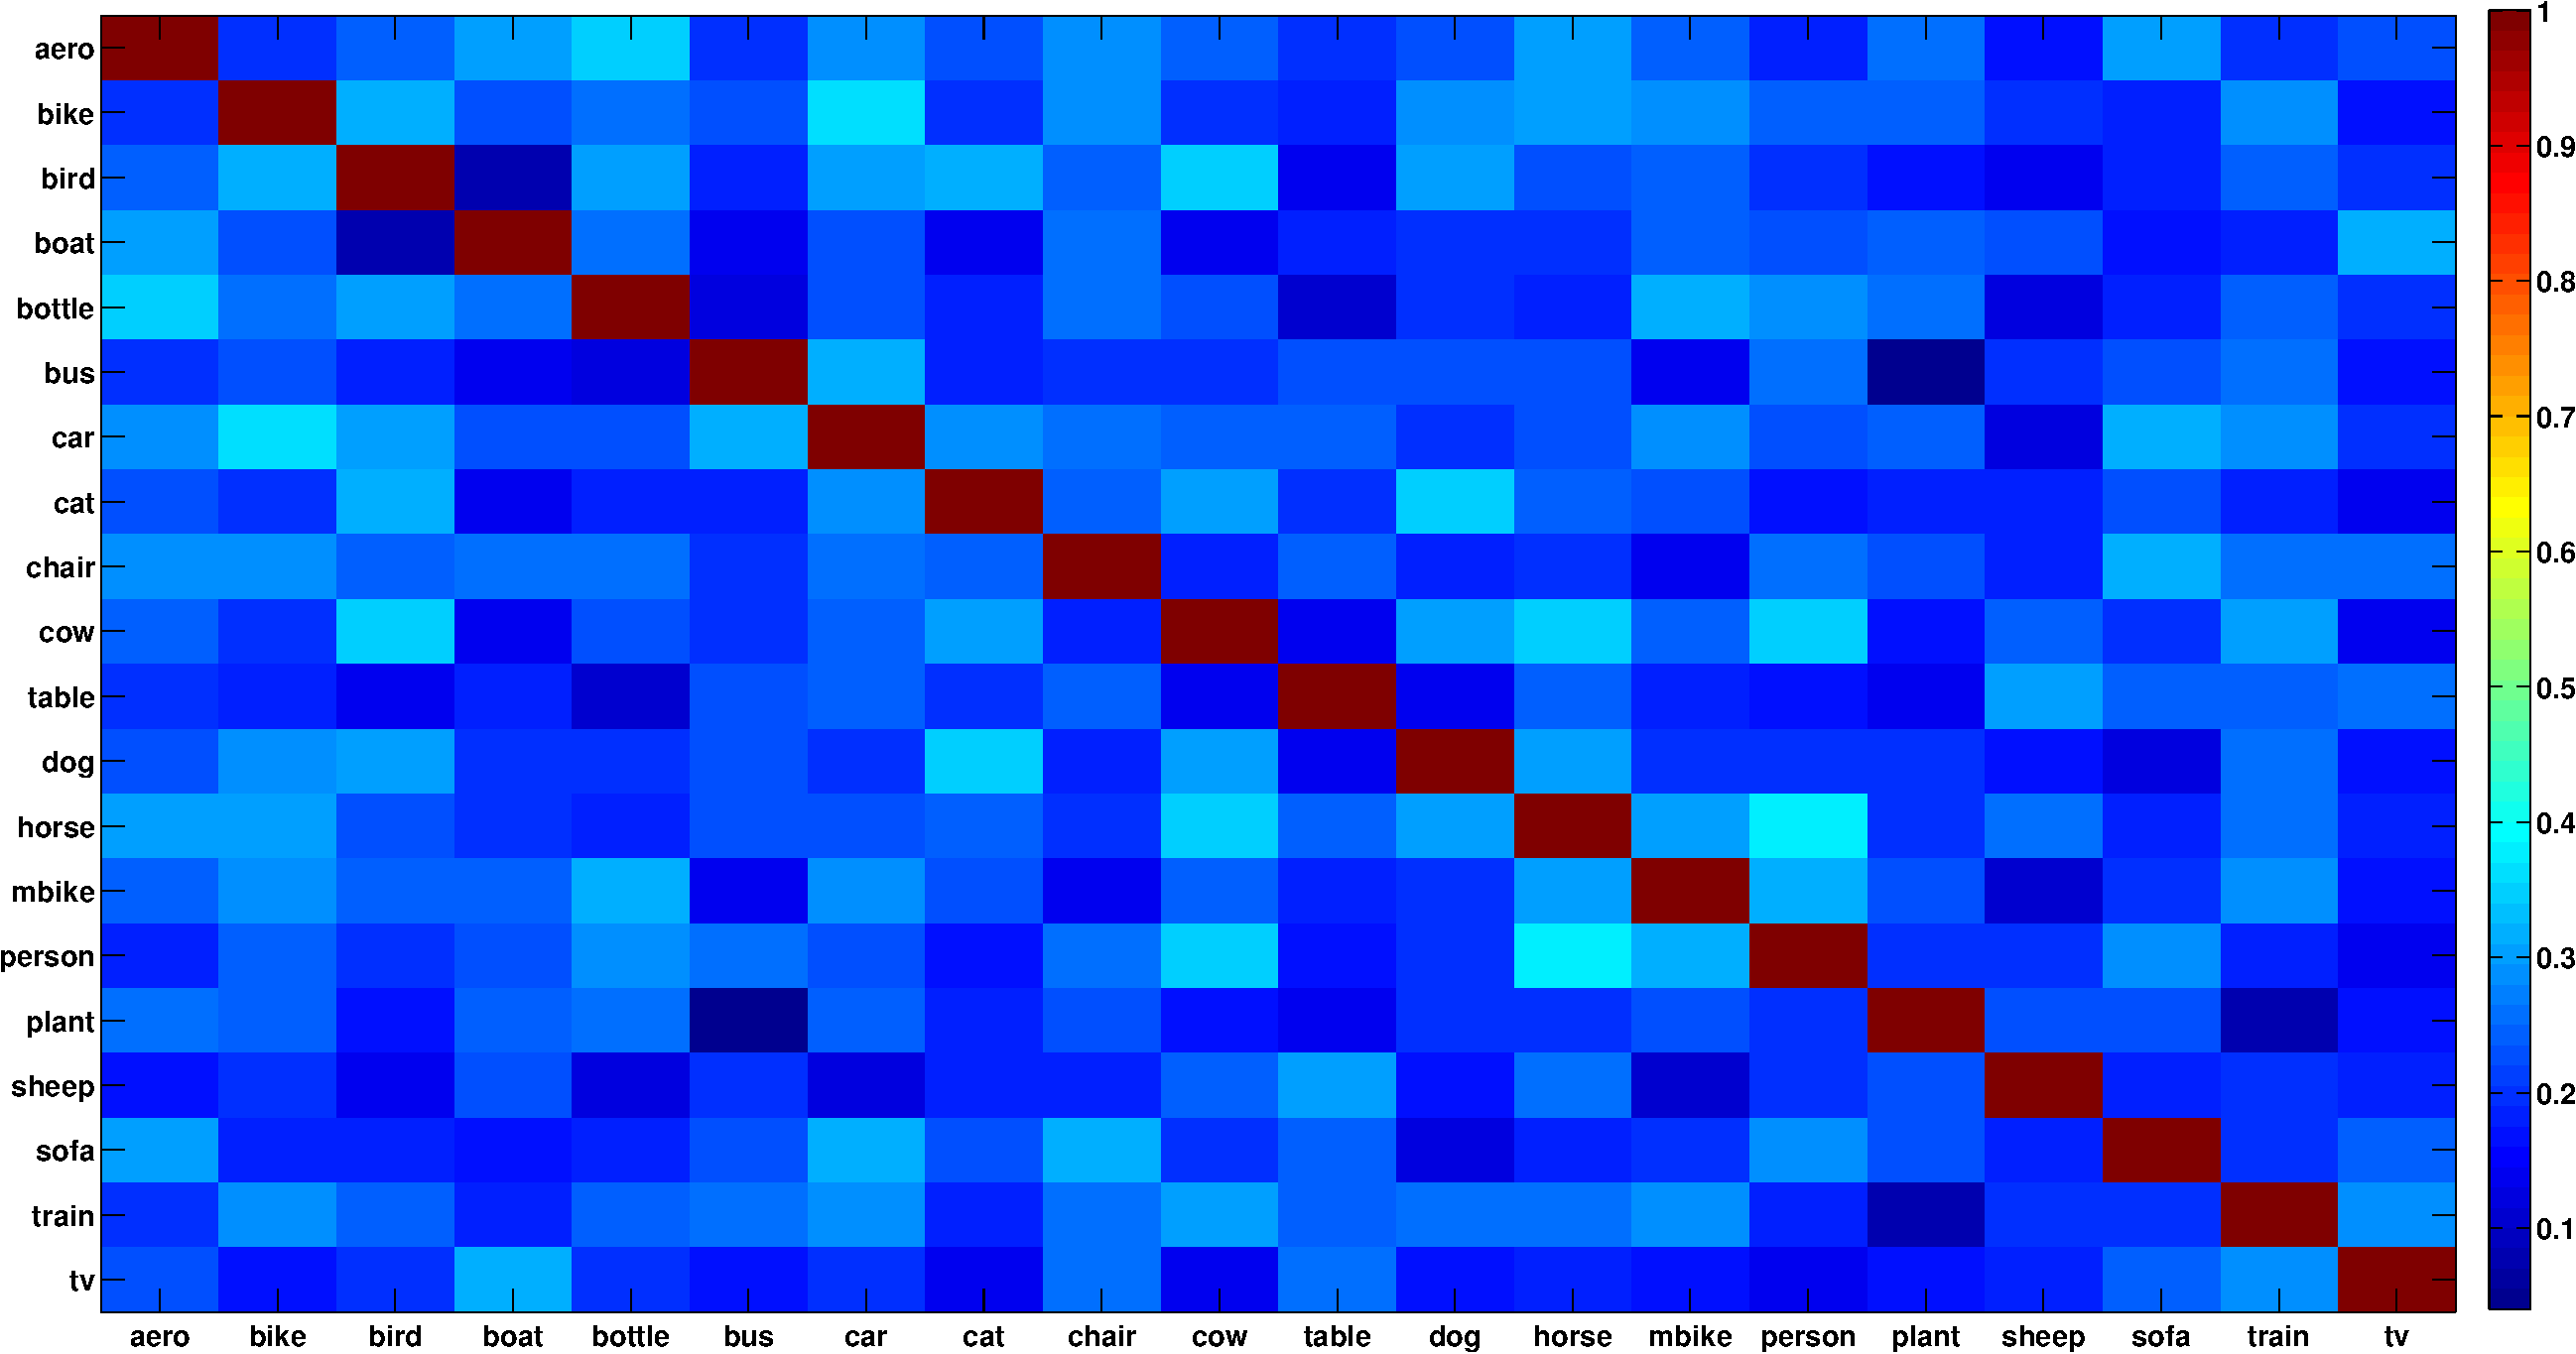
\includegraphics[width=1.0\linewidth]{images/FTNet_overlap.pdf}
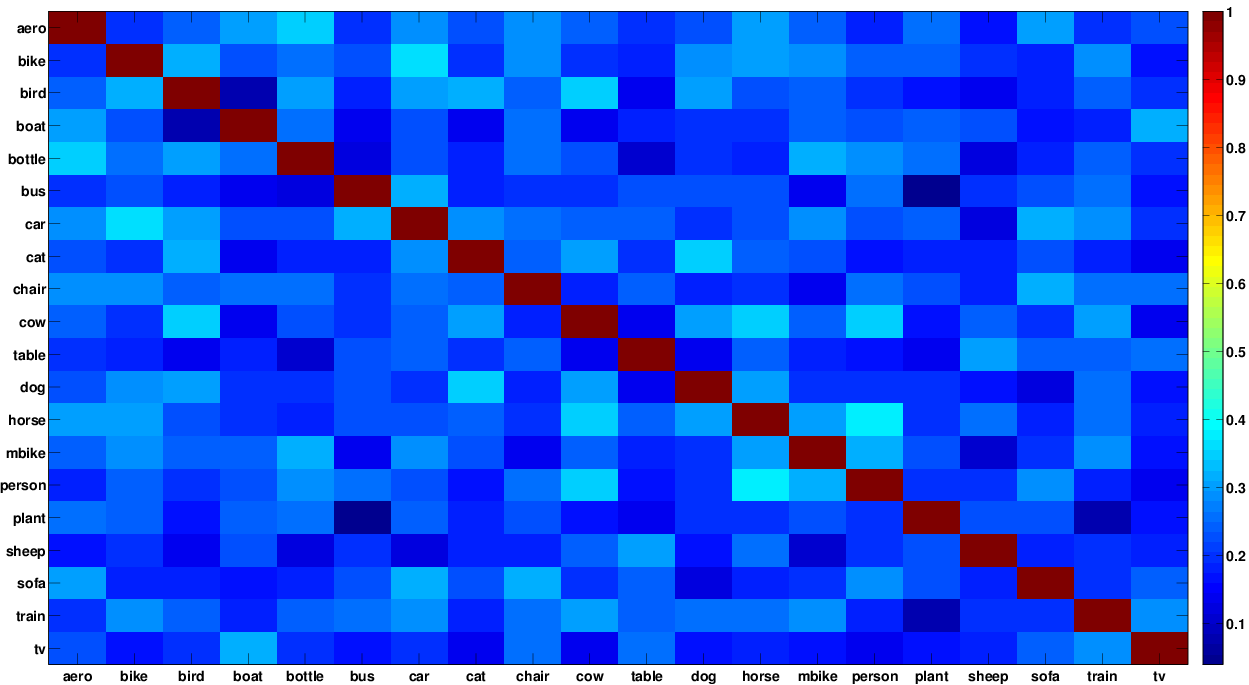
\includegraphics[width=1.0\linewidth]{images/ftNet.png}
\caption{The set overlap between the 50 most discriminative conv-5 filters for each class determined using PASCAL-DET-GT.
Entry $(i, j)$ of the matrix is the fraction of top-50 filters class $i$ has in common with class $j$ (Section \ref{sub:how-many}). Chance is 0.195. There is little overlap, but related classes are more likely to share filters.}
\label{fig:overlap}
\end{figure}

Next, we estimated the extent of overlap between the filters used for discriminating between different classes.
For each class $i$, we selected the 50 most discriminative filters (out of 256) and stored the selected filter indices in the set $S_i$.
The extent of overlap between class $i$ and $j$ was evaluated by $|S_i \cap S_j| / N$,
where $N = |S_i| = |S_j| = 50$. The results are visualized in Figure \ref{fig:overlap}. It can be seen that different classes use different subsets of conv-5 filters and there is little overlap between classes. This further indicates that intermediate representations in the CNN are distributed.
%and different sets of are used to distinguish between different classes. 
